\documentclass[11pt,a4paper,oneside]{book}
\usepackage[a4paper,margin=.78in,headheight=17pt,headsep=14pt,footskip=24pt]{geometry}
\usepackage{fontspec,graphicx,xcolor,fancyhdr,titlesec,enumitem,booktabs,longtable}
\usepackage[most]{tcolorbox}\usepackage{listings,tikz}\usetikzlibrary{arrows.meta,positioning}\usepackage[hidelinks]{hyperref}
\definecolor{Navy}{HTML}{15345B}\definecolor{Teal}{HTML}{148A8A}\definecolor{Gold}{HTML}{D9A441}\definecolor{Pale}{HTML}{EEF5F7}\definecolor{CodeBG}{HTML}{F4F7FA}
\setmainfont{TeX Gyre Pagella}\setlength{\parindent}{0pt}\setlength{\parskip}{4pt}
\setlist[itemize]{leftmargin=18pt,itemsep=2pt}\setlist[enumerate]{leftmargin=21pt,itemsep=2pt}
\titleformat{\chapter}[display]{\normalfont\bfseries\color{Navy}}{\Large\color{Teal}Chapter \thechapter}{3pt}{\huge}\titlespacing*{\chapter}{0pt}{-16pt}{9pt}
\titleformat{\section}{\large\bfseries\color{Teal}}{\thesection}{.6em}{}\titlespacing*{\section}{0pt}{8pt}{3pt}
\pagestyle{fancy}\fancyhf{}\fancyhead[L]{\small\textcolor{Navy}{Junior Software Developer — Grade XII}}\fancyhead[R]{\small\textcolor{Teal}{\leftmark}}\fancyfoot[L]{\small\textcolor{Navy}{Learning Handbook}}\fancyfoot[R]{\textcolor{Navy}{\thepage}}\renewcommand{\headrulewidth}{.6pt}
\lstset{basicstyle=\ttfamily\small,backgroundcolor=\color{CodeBG},frame=single,rulecolor=\color{Teal},breaklines=true,showstringspaces=false,keywordstyle=\color{Navy}\bfseries,commentstyle=\color{Teal},numbers=left,numberstyle=\tiny,xleftmargin=5pt,aboveskip=5pt,belowskip=5pt}
\newtcolorbox{keybox}[1][]{colback=Pale,colframe=Teal,boxrule=.7pt,arc=2mm,left=7pt,right=7pt,top=5pt,bottom=5pt,#1}
\newcommand{\photo}[3]{\begin{figure}[htbp]\centering\fcolorbox{Teal}{white}{\includegraphics[width=.78\linewidth,height=5cm,keepaspectratio]{images/#1}}\par\vspace{3pt}{\small\textbf{\textcolor{Navy}{#2}}}\par{\footnotesize #3}\end{figure}}
\newcommand{\review}[1]{\begin{keybox}[title={Review questions}]\begin{enumerate}#1\end{enumerate}\end{keybox}}
\begin{document}
\begin{titlepage}\thispagestyle{empty}
\begin{tikzpicture}[remember picture,overlay]\fill[Navy] (current page.north west) rectangle ([yshift=-5.2cm]current page.north east);\fill[Teal] ([yshift=-5.2cm]current page.north west) rectangle ([yshift=-5.36cm]current page.north east);\draw[Gold,line width=2pt] ([xshift=1cm,yshift=-1cm]current page.north west) rectangle ([xshift=-1cm,yshift=1cm]current page.south east);\end{tikzpicture}
\vspace*{1.2cm}\begin{center}{\Large\bfseries\color{white} VOCATIONAL LEARNING HANDBOOK}\\[1cm]{\Huge\bfseries\color{white} JUNIOR SOFTWARE}\\[2pt]{\Huge\bfseries\color{white} DEVELOPER}\\[.3cm]{\Large\bfseries\color{Gold} GRADE XII}\\[1.3cm]
\begin{tcolorbox}[width=.8\linewidth,colback=white,colframe=Gold,arc=3mm]\centering\Large\bfseries\color{Navy} RDBMS and SQL \textbullet\ Advanced Python\\[3pt] Software Engineering \textbullet\ Emerging Technologies\end{tcolorbox}
\vfill\includegraphics[width=.65\linewidth,height=4.3cm,keepaspectratio]{images/motherboard.jpg}\\[.5cm]{\large\bfseries\color{Navy} CONCEPTS \quad PRACTICE \quad APPLICATION}\\[.4cm]{\small A textbook-style learning companion aligned to the Grade XII topic outline}\vspace*{1.2cm}\end{center}\end{titlepage}
\frontmatter
\chapter*{About this handbook}
This handbook follows the four topic areas in the supplied Grade XII Junior Software Developer study material: relational database concepts and MySQL; advanced Python; software engineering; and emerging technologies with social impact. Explanations, examples and exercises are freshly written for study and revision.
\begin{keybox}\textbf{Study method.} Read the concept, trace the example, run code in a safe environment, modify one input, then answer the review questions without looking back.\end{keybox}
\tableofcontents\mainmatter
\chapter{Relational Database Foundations}
\section{Data and information}
Data are recorded facts such as student numbers, prices, dates or quantities. Information is data arranged to answer a question. A database is an organised collection of related data that can be searched and updated consistently. A database management system (DBMS) defines, stores, retrieves and protects data. A relational DBMS represents data through tables of rows and columns.
\section{File systems and databases}
Independent files may duplicate values and become inconsistent when only some copies are updated. A DBMS supports controlled access, validation, shared data, backup and query-based retrieval. These benefits depend on sound design and configuration.
\begin{center}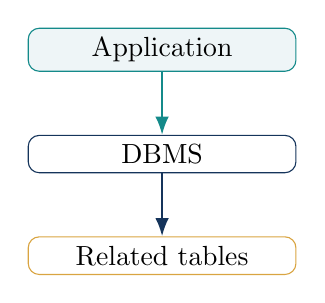
\begin{tikzpicture}[node distance=8mm,>=Latex]\node[draw=Teal,fill=Pale,rounded corners,minimum width=3.4cm] (a) {Application};\node[draw=Navy,rounded corners,minimum width=3.4cm,below=of a] (b) {DBMS};\node[draw=Gold,rounded corners,minimum width=3.4cm,below=of b] (c) {Related tables};\draw[->,thick,Teal](a)--(b);\draw[->,thick,Navy](b)--(c);\end{tikzpicture}\end{center}
\section{Tables, keys and constraints}
A relation is a table; a tuple is a row; an attribute is a column; a domain is the set of valid values; a schema is the planned structure; an instance is the data present at a particular time. A candidate key uniquely identifies a row. One candidate becomes the primary key. A composite key combines attributes. A foreign key references a key in another table. Constraints such as NOT NULL, UNIQUE and CHECK express rules close to the data.
\begin{center}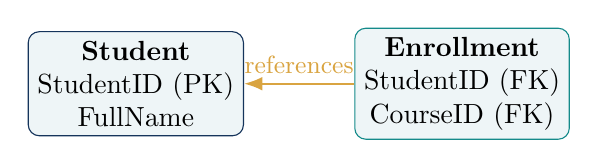
\begin{tikzpicture}[node distance=14mm,>=Latex]\node[draw=Navy,fill=Pale,rounded corners,align=center] (s) {\textbf{Student}\\StudentID (PK)\\FullName};\node[draw=Teal,fill=Pale,rounded corners,align=center,right=of s] (e) {\textbf{Enrollment}\\StudentID (FK)\\CourseID (FK)};\draw[->,thick,Gold](e.west)--node[above,font=\small]{references}(s.east);\end{tikzpicture}\end{center}
\section{Database models}
Relational databases use related tables. Document stores hold document-like records; key-value stores map keys to values; graph databases emphasise relationships. Select a model based on data shape, consistency needs and query patterns.
\review{\item Explain data versus information.\item Give four limitations of independent file-based records.\item Define relation, tuple, attribute, schema and instance.\item Distinguish primary and foreign keys.\item Give one relational database use case.}
\chapter{SQL: Defining and Manipulating Data}
\section{SQL command families}
SQL defines database structures, changes records, retrieves information and controls access. DDL includes CREATE, ALTER and DROP; DML includes INSERT, UPDATE and DELETE; SELECT retrieves records; DCL manages permissions; TCL includes COMMIT and ROLLBACK.
\section{Create, insert and retrieve}
\begin{lstlisting}[language=SQL]
CREATE DATABASE training;
USE training;
CREATE TABLE Student (
  StudentID INT PRIMARY KEY,
  FullName VARCHAR(80) NOT NULL,
  ClassLevel TINYINT NOT NULL,
  Email VARCHAR(120) UNIQUE
);
INSERT INTO Student (StudentID, FullName, ClassLevel)
VALUES (1204, 'Anu Rao', 12);
SELECT StudentID, FullName
FROM Student
WHERE ClassLevel = 12
ORDER BY FullName;
\end{lstlisting}
Choose types deliberately. Use date types for dates, suitable text types for names and exact decimal types for currency. WHERE filters rows; ORDER BY sorts; GROUP BY forms groups; HAVING filters groups after aggregation.
\begin{lstlisting}[language=SQL]
SELECT ClassLevel, COUNT(*) AS StudentCount
FROM Student
GROUP BY ClassLevel
HAVING COUNT(*) >= 5
ORDER BY StudentCount DESC;
\end{lstlisting}
\section{Joins and transactions}
An inner join returns matching rows; a left join retains all rows from the left table. A transaction groups changes into one logical unit. ACID describes atomicity, consistency, isolation and durability. Check the condition of UPDATE or DELETE with SELECT first. Use parameterised queries in applications instead of concatenating untrusted input.
\photo{programming-code.png}{Reading structured code}{A code editor is a practical place to inspect SQL and application logic. Image source and licence are listed in IMAGE-CREDITS.txt.}
\review{\item Explain DDL and DML with examples.\item Write a query to retrieve Grade XII students alphabetically.\item Distinguish WHERE and HAVING.\item What is a join?\item Why are parameterised queries important?}
\chapter{SQL Functions and Relational Design}
Single-row functions transform values per row. String functions change case or measure text; numeric functions round values; date functions work with calendar values. Aggregate functions such as COUNT, SUM, AVG, MIN and MAX summarise groups. COUNT(column) generally excludes null values, while COUNT(*) counts rows.
\begin{lstlisting}[language=SQL]
SELECT UPPER(FullName) AS DisplayName,
       CHAR_LENGTH(FullName) AS NameLength
FROM Student;
\end{lstlisting}
Normalisation reduces duplication and update anomalies. First normal form expects atomic values and no repeating groups. Second normal form removes partial dependencies on part of a composite key. Third normal form removes inappropriate transitive dependencies among non-key attributes.
\begin{keybox}If an order table repeats a supplier address on every row, corrections require many updates. A separate Supplier table referenced by a key reduces duplication.\end{keybox}
\review{\item Distinguish single-row and aggregate functions.\item Why can COUNT(*) differ from COUNT(Email)?\item What is an update anomaly?\item Explain normalisation.\item List the main database design steps.}
\chapter{Python Data Structures: Stack and Queue}
A stack follows last-in, first-out (LIFO); the last item added is removed first. A queue follows first-in, first-out (FIFO); the earliest item is removed first. Stacks suit undo histories and function calls; queues suit print jobs and service requests.
\photo{stack-queue.png}{Stack and queue comparison}{The structures differ in the order items leave the collection. Source and licence are listed in IMAGE-CREDITS.txt.}
\begin{lstlisting}[language=Python]
from collections import deque
stack = []
stack.append("first")
stack.append("second")
print(stack.pop())       # second
queue = deque(["first", "second"])
queue.append("third")
print(queue.popleft())   # first
\end{lstlisting}
Use deque for efficient queue operations. Test empty structures and decide how to handle attempts to remove an item when none exists.
\review{\item Define LIFO and FIFO.\item Give two uses of each structure.\item Why is deque useful for queues?\item How should an empty-stack pop be handled?}
\chapter{Exception Handling in Python}
A syntax error prevents parsing; a runtime exception occurs during execution; a logic error produces an incorrect result even though the program runs. Use try for risky operations, except for expected exception types, else for success-only actions and finally for cleanup.
\begin{lstlisting}[language=Python]
raw = input("Enter a whole number: ")
try:
    value = int(raw)
except ValueError:
    print("Please enter a valid whole number.")
else:
    print("Double:", value * 2)
finally:
    print("Input attempt finished.")
\end{lstlisting}
Catch the narrowest useful exception. Avoid broad handlers that hide defects. Raise an exception when an input violates a function's documented contract.
\review{\item Distinguish syntax, runtime and logic errors.\item Explain else and finally.\item Why avoid bare except clauses?\item Write an example handling ValueError.}
\chapter{File Handling in Python}
Text files store characters; binary files store bytes. Modes include r for reading, w for replacing content, a for appending and x for exclusive creation. The with statement closes files reliably after a block.
\begin{lstlisting}[language=Python]
with open("notes.txt", "w", encoding="utf-8") as file:
    file.write("Python file handling\n")
with open("notes.txt", "r", encoding="utf-8") as file:
    print(file.read())
\end{lstlisting}
CSV stores rows and columns; Python's csv module handles quoted values. JSON represents objects, arrays and primitive values and is commonly used by APIs. Validate user-provided files, avoid overwriting valuable data without backups and never commit secrets to source control.
\begin{lstlisting}[language=Python]
import csv
with open("marks.csv", newline="", encoding="utf-8") as file:
    for row in csv.DictReader(file):
        print(row.get("StudentName"), row.get("Marks"))
\end{lstlisting}
\review{\item Distinguish w and a modes.\item Why is with open preferred?\item Why use the csv module?\item Give two file-safety precautions.}
\chapter{NumPy Arrays}
NumPy supports multidimensional arrays and numerical operations. Arrays usually contain values of a common type and support vectorised calculations.
\begin{lstlisting}[language=Python]
import numpy as np
marks = np.array([72, 81, 69, 94])
print(marks.mean())
print(marks.max())
print(marks[1:3])
print(marks.shape, marks.ndim, marks.dtype)
\end{lstlisting}
Shape describes dimensions, ndim gives the number of dimensions and dtype reports the element type. Vectorisation applies operations to whole arrays. Broadcasting allows compatible shapes to work together; check shapes to avoid unintended calculations.
\review{\item Compare lists and NumPy arrays.\item Explain shape, ndim and dtype.\item What is vectorisation?\item Why check array shapes?}
\chapter{Pandas and Series}
Pandas provides labelled structures for cleaning and analysing tabular data. A Series is a one-dimensional labelled sequence; a DataFrame is a table-like structure.
\begin{lstlisting}[language=Python]
import pandas as pd
data = pd.DataFrame({
    "student": ["Asha", "Ravi", "Meena"],
    "marks": [82, 76, 91]
})
print(data.head())
print(data["marks"].mean())
print(data.describe())
\end{lstlisting}
Use column names to select values and Boolean conditions to filter rows. Inspect missing values with isna(); remove or fill them only when justified. Grouping summarises categories. Before merging, check key uniqueness because many-to-many joins may multiply rows.
\review{\item Distinguish Series and DataFrame.\item How can missing values be inspected?\item Why might a merge increase row count?\item Describe a simple marks analysis.}
\chapter{Visualisation with Matplotlib}
Bar charts compare categories; line charts show change over an ordered scale; scatter plots explore numeric relationships; histograms show distributions.
\photo{python-simulation.jpg}{Python code and plotted output}{A programming environment can connect calculations with visual interpretation; see IMAGE-CREDITS.txt.}
\begin{lstlisting}[language=Python]
import matplotlib.pyplot as plt
subjects = ["SQL", "Python", "Networks"]
scores = [78, 86, 74]
plt.bar(subjects, scores)
plt.title("Practice assessment scores")
plt.xlabel("Subject")
plt.ylabel("Score")
plt.ylim(0, 100)
plt.tight_layout()
plt.show()
\end{lstlisting}
Label axes and units, use readable scales and explain the data source. Avoid decoration that distorts comparisons or implies unsupported precision.
\review{\item Match chart types to questions.\item Why label axes?\item Name two ways charts can mislead.\item Outline steps to create a bar chart.}
\chapter{Connecting Python with MySQL}
A database connector lets Python send SQL statements and receive results. A typical workflow loads configuration securely, opens a connection, creates a cursor, executes parameterised statements, commits successful changes, rolls back failures and closes resources.
\begin{lstlisting}[language=Python]
# Illustrative pattern; configure a MySQL connector first.
sql = "SELECT StudentID, FullName FROM Student WHERE ClassLevel = %s"
cursor.execute(sql, (12,))
rows = cursor.fetchall()
for row in rows:
    print(row)
\end{lstlisting}
Placeholder syntax depends on the connector. Keep credentials outside source code, grant least privilege, handle network failures and avoid exposing sensitive records in logs.
\review{\item Describe the Python-to-MySQL workflow.\item Why use parameterised statements?\item Explain commit and rollback.\item Give three ways to protect credentials.}
\chapter{Software Engineering Concepts}
Software engineering applies systematic methods to build, test, release and maintain software. Functional requirements describe actions the system must perform. Non-functional requirements describe qualities such as response time, security, availability and accessibility. Requirements should be testable and unambiguous.
\begin{keybox}\textbf{Vague:} The report should be fast. \textbf{Measurable:} For 10,000 records in the stated environment, 95 percent of report requests should complete within two seconds.\end{keybox}
Modularity divides a system into components with clear responsibilities. High cohesion means a component's tasks belong together; low coupling limits unnecessary dependencies. Quality attributes include reliability, maintainability, portability, scalability, usability and security.
\review{\item Distinguish functional and non-functional requirements.\item Define cohesion and coupling.\item List five quality attributes.\item Rewrite a vague requirement measurably.}
\chapter{Software Development Life Cycle}
Typical activities include planning, requirements analysis, design, implementation, testing, deployment and maintenance. Sequential and iterative approaches organise these activities differently; feedback may send work back to earlier stages.
\begin{center}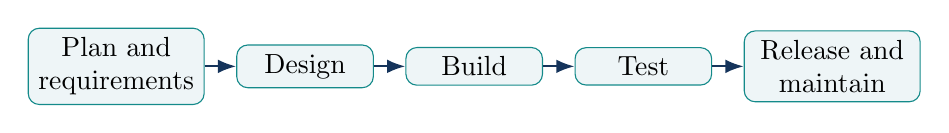
\begin{tikzpicture}[node distance=4mm and 4mm,>=Latex]\node[draw=Teal,fill=Pale,rounded corners,align=center,text width=2cm] (a) {Plan and\\requirements};\node[draw=Teal,fill=Pale,rounded corners,align=center,text width=1.5cm,right=of a] (b) {Design};\node[draw=Teal,fill=Pale,rounded corners,align=center,text width=1.5cm,right=of b] (c) {Build};\node[draw=Teal,fill=Pale,rounded corners,align=center,text width=1.5cm,right=of c] (d) {Test};\node[draw=Teal,fill=Pale,rounded corners,align=center,text width=2cm,right=of d] (e) {Release and\\maintain};\draw[->,thick,Navy](a)--(b);\draw[->,thick,Navy](b)--(c);\draw[->,thick,Navy](c)--(d);\draw[->,thick,Navy](d)--(e);\end{tikzpicture}\end{center}
Plan-driven methods suit some stable or constrained projects. Iterative methods deliver increments and incorporate feedback. Version control records changes; meaningful commits and code review support collaboration. Risk planning records likelihood, impact, owners and mitigation actions.
\review{\item List typical SDLC activities.\item Compare plan-driven and iterative approaches.\item Why is code review useful?\item Describe a project risk and mitigation.}
\chapter{Software Testing and Maintenance}
Unit tests check small components; integration tests check interactions; system tests assess the full product; acceptance tests assess user needs. Regression tests check that a change has not broken existing behaviour. A test case defines inputs, preconditions, actions and expected results. Include typical values, boundaries, invalid inputs and failure conditions.
Debug systematically: reproduce the issue, gather evidence, narrow the cause, make a fix and rerun relevant tests. Deployment planning includes configuration, database migration, monitoring and rollback.
\begin{keybox}For a function accepting marks from 0 to 100, test 0, 100, a normal value, below 0, above 100 and non-numeric input.\end{keybox}
\review{\item Explain unit, integration, system and acceptance testing.\item What is regression testing?\item Why test boundary values?\item Outline a safe debugging process.\item What belongs in a rollback plan?}
\chapter{Emerging Technologies}
AI includes systems for perception, language, prediction or planning. Machine learning uses data to fit patterns. Generative AI produces text, images, code or audio. Outputs can be inaccurate or biased; evaluate them and keep human oversight for consequential decisions.
Cloud computing offers on-demand computing, storage, databases and software. IaaS provides infrastructure, PaaS a managed platform and SaaS a ready-to-use application. Internet of Things devices combine sensors, software and connectivity. Edge computing processes data near its source, potentially reducing latency.
Blockchain is a shared ledger maintained using a consensus mechanism; it is not automatically private or suitable for every database problem. Augmented reality overlays digital information on the physical world; virtual reality immerses users in a simulated environment. Robotic process automation performs repetitive rule-based tasks but needs controls for exceptions and auditability.
\review{\item Distinguish AI, ML and generative AI.\item Compare IaaS, PaaS and SaaS.\item When might edge computing help?\item Give one limitation of blockchain.\item Name a responsible AI safeguard.}
\chapter{Social Impact, Ethics and Cyber Safety}
Technology can expand access but may exclude people due to cost, connectivity, language, disability or limited digital skills. Accessible design considers keyboard use, contrast, captions and assistive technology. Collect only necessary personal data, restrict access and protect it in storage and transfer.
Cyber safety includes unique passwords, multifactor authentication, timely updates, backups and caution with unexpected links. Phishing attempts to trick people into disclosing information or running unsafe actions. Respect copyright, software licences, privacy and attribution. Consider energy use, repairability, device lifespan and responsible e-waste disposal.
\review{\item Define digital inclusion.\item List five principles for responsible data handling.\item Give common phishing warning signs.\item Why do software licences and image credits matter?\item Suggest three sustainable computing practices.}
\chapter{Integrated Practical Project}
Design a small student learning-record system using fictional data only. Write functional requirements for adding a student, recording a score and producing a class summary. Add non-functional requirements for access control, clarity and recovery. Design tables with primary and foreign keys, create test data and query averages and counts.
Use Python to process results and create a labelled chart. Separate database access, validation and presentation into functions. Prepare normal, boundary and invalid-input tests, record expected and actual results, document setup and limitations, and identify privacy risks.
\review{\item Draw a basic entity relationship model.\item Write two functional and two non-functional requirements.\item Propose five test cases.\item Explain how Python and SQL work together.\item Identify two privacy risks and mitigations.}
\chapter{Revision and Key Terms}
\begin{longtable}{p{.25\linewidth}p{.67\linewidth}}\toprule\textbf{Area}&\textbf{Remember}\\\midrule
Relational databases&Tables, rows, attributes, keys, constraints, relationships and integrity.\\
SQL&Define structures, manipulate and retrieve records, join, group and manage transactions.\\
SQL functions&String, numeric, date and aggregate operations; null handling and normalisation.\\
Advanced Python&Stacks, queues, exceptions, files and resource management.\\
NumPy and Pandas&Arrays, shapes, labelled data, filtering, cleaning and aggregation.\\
Visualisation&Match chart type to question; label axes and avoid misleading scales.\\
Database connectivity&Parameterised queries, least privilege, transactions and secret management.\\
Software engineering&Requirements, modular design, lifecycle, collaboration, testing and maintenance.\\
Emerging technology&Assess benefit, maturity, cost, privacy, safety and limitations.\\
Social impact&Inclusion, accessibility, ethical data use, cyber safety, licences and sustainability.\\\bottomrule\end{longtable}
\begin{keybox}\textbf{Final self-check:} Can I explain concepts in my own words, test code safely, design related tables, evaluate evidence and identify security or ethical concerns?\end{keybox}
\backmatter
\chapter*{Image credits and publication note}
Image authors, licences and source pages are listed in the accompanying IMAGE-CREDITS.txt. This learning companion is freshly authored around the supplied topic outline and is not an official NCERT/PSSCIVE publication.
\end{document}
